% Provenance (never printed): old premiere S material on the history of plate
% tectonics (from continental drift to seafloor spreading: the ridges, the
% magnetic stripes, the ages of the drilled floor); see
% sources/book2/PROVENANCE.md. Profiles are computed in
% figdata/grade-11/magnetic_stripes.py, the age map in seafloor_age.py, the
% drilling fit in sediment_ages.py.
\chapter{من الانجراف القاري إلى توسع قاع المحيط}\label{ch:g11:drift-to-spreading}

في مطلع خمسينيات القرن العشرين، في مختبر لامونت التابع لجامعة كولومبيا، جلست
عالمة جيولوجيا شابة تدعى ماري ثارب أمام صفوف طويلة من الأرقام. كان كل رقم منها عمقًا
من أعماق شمال الأطلسي، قاسه مسبار الصدى في سفينة، رقمًا بعد رقم على طول مسار
السفينة. وبرسمها واحدًا واحدًا، خطّت شكل قاع المحيط على طول مسارات السفن التي
عبرت المحيط. ففي وسط المحيط يرتفع القاع سلسلةً جبلية --- وعلى كل مسار، على طول
قمة السلسلة، كان القاع ينخفض من جديد في شق عميق، كأن الجبال قد شُقّت من
وسطها. يتتبع هذا الفصل كيف حوّلت قياساتٌ كهذه لقاع المحيط فكرةً مرفوضة، هي انجراف
القارات، إلى نظرية: قاع المحيط يُصنع عند الظهرات ويتوسع مبتعدًا عنها، ويحمل في
صخوره سجلًا لعمره.
% ledger: aip:tharp, aip:featureless, usgs:echo-sounding

\begin{recall}
الانجراف القاري هو فكرة أن القارات تتحرك؛ وقد دافع عنها ألفريد فيغنر منذ عام 1912
بتطابق السواحل، والأحافير، والصخور، والمناخات القديمة، لكنه لم يستطع أن يقول ما الذي
يحركها. يتكون سطح الأرض من صفائح صلبة تلتقي عند حدود متباعدة ومتقاربة
وتحويلية؛ وهي تتحرك بضعة سنتيمترات في السنة، و$\qty{1}{cm}$ في السنة يساوي $\qty{10}{km}$
في كل مليون سنة (الكتاب 1، الصف 7). ولقاع المحيط رفه
القاري، وسهوله السحيقة، وظهراته، وخنادقه (الكتاب 1، الصف 8).
وللأرض مجال مغناطيسي، له قطب مغناطيسي شمالي وآخر جنوبي، تتبعه إبرة
البوصلة؛ ونبضة الصوت المرسلة في الماء تعود صدًى
بعد زمن يعطي المسافة (كتب الفيزياء).
\end{recall}

\section{لماذا رُفض الانجراف}

أظهرت أدلة فيغنر أن القارات كانت متصلة يومًا ما. أما ما لم تُظهره فهو كيف أمكنها
أن تتحرك. فقد تخيّل فيغنر القارات تشق طريقها عبر صخور قاع المحيط كما يشق المحراث
الأرض، فأجابه الفيزيائيون بأن لا قوة معروفة تستطيع دفع قارة عبر صخر
صلب دون أن تسحقها. وطوال نصف قرن خلص معظم الجيولوجيين إلى أن
القارات لم تتحرك قط.
% ledger: usgs:wegener-1912, usgs:jeffreys (Book 1 rows)

كان ثمة أمران ناقصان. الأول آلية. والثاني، وهو الذي قاد إلى
الأول، معرفة قاع المحيطات، الذي يغطي معظم سطح
الأرض والذي لم يكن أحد تقريبًا قد رآه في عام 1912: فقد افتُرض أنه
سهل يكاد يخلو من التضاريس.
% ledger: aip:tharp, aip:featureless

\section{رسم خريطة قاع المحيط}

يرسل مسبار الصدى نبضة قصيرة من الصوت من بدن السفينة إلى
قاع البحر ويقيس زمن عودة صداها. ينتقل الصوت في ماء البحر بسرعة تقارب
\qty{1500}{m/s}؛ والنبضة تنزل ثم تعود، فالتأخر $t$ يعني
عمقًا
\[
  d = \frac{v\,t}{2}.
\]
فتأخر قدره \qty{6.0}{s}، مثلًا، يعني $1500 \times 6.0/2 =
\qty{4500}{m}$ من الماء. وفي القرن التاسع عشر كانت الأعماق تقاس واحدًا
واحدًا، بإنزال حبل مثقل حتى القاع. وبعد الحرب العالمية
الأولى حلّت مسابير الصدى محله، فأظهرت سجلات أصدائها قاعًا
أشد وعورة بكثير مما ظنه أي أحد؛ وفي الخمسينيات أظهرت مسوح سفن من أمم كثيرة أن
سلسلة جبلية عظيمة في قاع المحيط تلتف حول الأرض كلها
تقريبًا.
% ledger: noaa:sound-seawater, usgs:echo-sounding, usgs:line-soundings

\begin{history}[ماري ثارب ووادي الخسف، 1952]
% ledger: aip:tharp, aip:featureless
منذ عام 1947 كان الجيوفيزيائي بروس هيزن قد جمع مقاطع سبر بالصدى
عبر شمال الأطلسي. وحوّلت ماري ثارب، التي لم يكن يُسمح لها آنذاك بركوب سفن
البحث، ما سمّته لاحقًا «صفوفًا لا تنتهي من أرقام
السبر» إلى رسوم لقاع البحر. وبحلول عام 1952، بعد أن رتّبت المسارات الممتدة من الشرق
إلى الغرب من الشمال إلى الجنوب، رأت أن معلمًا واحدًا يصطف
من مسار إلى مسار: شقًّا على طول قمة ظهرة وسط الأطلسي، أي واديًا
خسفيًا. وظن هيزن أول الأمر أنه خطأ. ثم تبيّن أن المراكز السطحية
لزلازل الأطلسي، حين رُسمت بالمقياس نفسه، تقع في وادي
الخسف نفسه. وقد أعطت خريطة ثارب وهيزن لقاع المحيطات في العالم،
التي رسمها الفنان هاينريش برّان عام 1977، الناس أول صورة واقعية لقاع المحيط؛ وفي عام 1997
عدّتها مكتبة الكونغرس واحدة من أعظم أربعة رسامي خرائط في
القرن العشرين.
\end{history}

تشكّل الظهرات وسط المحيطية منظومة واحدة شبه متصلة طولها نحو
\qty{65000}{km}، يقع أكثر من تسعة أعشارها تحت الماء؛ وتقع القمة
في المتوسط على عمق \qty{2500}{m} تحت السطح. وعلى طول ظهرة وسط الأطلسي البطيئة،
يشق القمةَ وادي خسف؛ أما على طول ظهرة شرق المحيط الهادئ الأسرع فهي
قمة ملساء لطيفة الانحدار. وتتبع زلازل المحيطات الظهرات
عن قرب. كان كل شيء يشير إلى أن الظهرة مكان
يحدث فيه شيء ما --- ولكن ما هو؟
% ledger: noaa:ridge, aip:tharp

\section{توسع قاع المحيط}

\begin{history}[هس والحزام الناقل، 1962]
% ledger: usgs:hess, hess:1962
في عام 1962 نشر هاري هس، وهو جيولوجي في جامعة برينستون وأميرال في
الاحتياط البحري، بحثه \emph{«تاريخ أحواض المحيطات»}.
واقترح أن صخرًا ساخنًا يصعد تحت الظهرات ويصير قاعًا محيطيًا جديدًا،
ثم يبتعد على الجانبين كأنه حزام ناقل، ويغوص عائدًا إلى
الوشاح عند الخنادق. وأعطى روبرت ديتز، الذي توصّل إلى الفكرة نفسها، هذه الفكرة
اسمها: \omterm{def:g11:drift-to-spreading:spreading}{توسع قاع المحيط}. وقد فسّرت الفكرة لماذا لا تكبر الأرض
مع أن قاعًا جديدًا يُصنع دائمًا، ولماذا لا يوجد إلا القليل من الرواسب على
قاع المحيط، ولماذا تكون صخور قاع المحيط أحدث بكثير من صخور
القارات.
\end{history}

\begin{definition}[توسع قاع المحيط]\label{def:g11:drift-to-spreading:spreading}
\emph{توسع قاع المحيط}\index{توسع قاع المحيط} هو العملية التي يتكوّن بها
قاع محيطي جديد على طول قمة ظهرة وسط محيطية، حيث يصعد صخر منصهر
من الوشاح ويتصلب، ثم يبتعد عن الظهرة على
الجانبين، فيزداد قاع المحيط قِدمًا كلما ابتعد عن الظهرة.
\end{definition}

\begin{definition}[معدل التوسع]\label{def:g11:drift-to-spreading:spreading-rate}
\emph{معدل التوسع الكلي}\index{معدل التوسع} لظهرة هو السرعة التي
تتباعد بها الصفيحتان الواقعتان على جانبيها. و\emph{نصف معدل
التوسع} هو السرعة التي يبتعد بها القاع على أحد الجانبين عن محور
الظهرة. وحين يكون التوسع متماثلًا، يكون المعدل الكلي ضعف نصف المعدل.
\end{definition}

تتوسع الظهرات بسرعات شديدة التفاوت. فظهرة وسط الأطلسي تنفتح بمعدل
\qtyrange{2}{5}{cm} في السنة، وظهرة شرق المحيط الهادئ بمعدل \qtyrange{6}{16}{cm} في
السنة. ومن قاع المحيط الموجود اليوم، صُنع نحو الثلث عند ظهرات
بطيئة (معدلات كلية من \qtyrange{20}{55}{mm} في السنة) ونحو الخُمسين عند
ظهرات سريعة (\qtyrange{75}{180}{mm} في السنة).
% ledger: noaa:ridge, seton:rate-classes

كانت فكرة هس جريئة، ولم يكن لها في البداية إلا القليل من الأدلة المباشرة. وقد جاءت الأدلة
من جهتين غير متوقعتين: مغناطيسية قاع المحيط
ورواسبه.

\section{الانقلابات المغناطيسية وقاع البحر المخطط}

\subsection{صخر يتذكر المجال}

يحتوي بازلت قاع المحيط حبيبات صغيرة من المغنتيت، وهو أكسيد
حديد شديد المغناطيسية. وحين تنبثق لابة البازلت تكون أسخن بكثير من أن
تحتفظ بأي مغنطة دائمة؛ ومع تبردها تتمغنط الحبيبات
موازيةً لمجال الأرض المحيط بها، ثم يُقفل ذلك الاتجاه
في الصخر.
% ledger: usgs:magnetometers

\begin{definition}[المغنطة المتبقية؛ درجة حرارة كوري]\label{def:g11:drift-to-spreading:remanence}
\emph{درجة حرارة كوري}\index{درجة حرارة كوري} لمعدن مغناطيسي هي
درجة الحرارة التي لا يستطيع فوقها أن يحتفظ بمغنطة خاصة به: نحو
\qty{580}{\celsius} للمغنتيت. والصخر الذي تبرد حبيباته المغناطيسية مجتازةً
درجة حرارة كوري في مجال الأرض يحتفظ بمغنطة موازية
لمجال ذلك الزمن، هي
\emph{المغنطة المتبقية}\index{مغنطة متبقية}. وهي تدوم طويلًا بعد أن يتغير المجال، ما لم يُسخَّن
الصخر من جديد فوق درجة حرارة كوري.
\end{definition}
% ledger: tarduno:curie

\begin{omfigure}
\begin{tikzpicture}[font=\footnotesize, >={Stealth[length=5pt]}]
  % ground and lava flow
  \fill[lith basalt] (0,0) rectangle (11,0.6);
  \fill[omLithBasalt!45!red!35] (0,0.6) -- (11,0.6) -- (11,1.9) .. controls (9,2.0) and (4,2.15) .. (0,2.05) -- cycle;
  \fill[omLithBasalt!70] (0,1.35) -- (11,1.25) -- (11,1.9) .. controls (9,2.0) and (4,2.15) .. (0,2.05) -- cycle;
  \draw[black!60] (0,1.35) -- (11,1.25);
  \draw[line width=0.8pt] (0,2.05) .. controls (4,2.15) and (9,2.0) .. (11,1.9);
  \draw[black!60] (0,0.6) -- (11,0.6);
  % field lines (northern hemisphere: pointing down to the north)
  \foreach \x in {0.6,2.4,4.2,6.0,7.8,9.6} {
    \draw[->, omDef, line width=0.9pt] (\x,4.0) -- (\x+1.1,2.55);
  }
  \node[anchor=south west, text=omDef] at (0.2,4.05) {المجال المغناطيسي للأرض};
  % locked grains in the cooled top
  \foreach \x in {0.5,1.3,...,10.5} {
    \draw[->, black, line width=0.6pt] (\x,1.86) -- (\x+0.25,1.53);
  }
  % random grains in the hot interior
  \foreach \x/\a in {0.6/20,1.5/140,2.3/250,3.2/80,4.0/310,4.9/190,5.7/40,6.6/120,7.4/280,8.3/20,9.1/200,10.0/330} {
    \draw[->, black!55, line width=0.5pt] (\x,0.95) -- ++(\a:0.22);
  }
  \node[anchor=west, align=left] at (11.15,1.75) {\foreignlanguage{arabic}{تبرد دون \babelsublr{\qty{580}{\celsius}}: تحتفظ}\\\foreignlanguage{arabic}{الحبيبات باتجاه المجال}};
  \node[anchor=west, align=left] at (11.15,0.92) {\foreignlanguage{arabic}{لا يزال فوق \babelsublr{\qty{580}{\celsius}}:}\\\foreignlanguage{arabic}{لا مغنطة دائمة}};
  \node[anchor=west, align=left] at (11.15,0.25) {صخر أقدم};
  \node[anchor=west] at (9.0,4.25) {الشمال $\rightarrow$};
\end{tikzpicture}

{\small لابة تبرد (رسم تخطيطي، في نصف الكرة الشمالي، حيث يتجه المجال
نحو الشمال وإلى الأسفل). لقد برد أعلى اللابة دون \omterm{def:g11:drift-to-spreading:remanence}{درجة حرارة كوري}
للمغنتيت: فحبيباتها المغناطيسية (الأسهم السوداء) تحتفظ
باتجاه المجال. أما الداخل، الذي لا يزال أسخن، فلا يسجل شيئًا بعد؛ وسوف
يسجل مجال اللحظة التي يبرد فيها.}
\end{omfigure}

\subsection{المجال ينقلب}

في أوائل القرن العشرين، وجد برنار برونهس (عام 1906) ثم موتونوري
ماتوياما (في العشرينيات) أن الصخور البركانية تنقسم إلى مجموعتين. ففي
بعضها تتجه المغنطة كما يتجه المجال الحالي؛ وفي الأخرى
تتجه في الاتجاه المعاكس، كأن القطبين المغناطيسيين الشمالي والجنوبي قد تبادلا
مكانيهما. لقد انقلب المجال نفسه، مرة بعد مرة.
% ledger: usgs:reversals

\begin{definition}[الانقلاب المغناطيسي؛ القطبية العادية والمعكوسة]\label{def:g11:drift-to-spreading:reversal}
\emph{الانقلاب المغناطيسي}\index{انقلاب مغناطيسي} هو تبادل
القطبين المغناطيسيين الشمالي والجنوبي للأرض. والزمن الذي كان المجال فيه يتجه كما
يتجه اليوم هو زمن \emph{قطبية عادية}\index{قطبية عادية}؛ والزمن
الذي كان يتجه فيه في الاتجاه المعاكس زمن \emph{قطبية
معكوسة}\index{قطبية معكوسة}. والصخر الذي تمغنط في أي من هذين الزمنين له
القطبية نفسها.
\end{definition}

تعطي اللابات المؤرخة تعاقب الفترات العادية والمعكوسة:
\emph{السلم الزمني للقطبية المغناطيسية الأرضية}. وتحمل فتراته الطويلة أسماء
علماء درسوا مغناطيسية الأرض (برونهس، وماتوياما، وغاوس،
وجلبرت)؛ أما الأحداث القصيرة داخلها فتحمل أسماء الأماكن التي
اكتُشفت فيها أول مرة.

\begin{omfigure}
\begin{tikzpicture}
\begin{axis}[width=0.92\linewidth, height=3.2cm, xmin=0, xmax=5.5, ymin=-0.9, ymax=1.9,
  axis y line=none, axis x line*=bottom, xtick={0,0.5,...,5.5}, tick label style={font=\small},
  xlabel={\foreignlanguage{arabic}{العمر بملايين السنين}}, label style={font=\small}, clip=false]
\addplot[fill=black, draw=none] table {figdata/out/grade-11-magnetic_stripes-timescale.dat};
\draw[black] (axis cs:0,0) rectangle (axis cs:5.5,1);
\begin{scope}[every node/.style={font=\scriptsize, anchor=south}]
  \node at (axis cs:0.39,1.05) {برونهس};
  \node at (axis cs:1.68,1.05) {ماتوياما};
  \node at (axis cs:3.08,1.05) {غاوس};
  \node at (axis cs:4.74,1.05) {جلبرت};
\end{scope}
\draw[black!60] (axis cs:0.78,1) -- (axis cs:0.78,1.45);
\draw[black!60] (axis cs:2.581,1) -- (axis cs:2.581,1.45);
\draw[black!60] (axis cs:3.58,1) -- (axis cs:3.58,1.45);
\begin{scope}[every node/.style={font=\scriptsize, anchor=north}]
  \node at (axis cs:1.03,-0.05) {هاراميو};
  \node at (axis cs:1.86,-0.05) {أولدوفاي};
\end{scope}
\node[font=\scriptsize, anchor=west] at (axis cs:5.55,0.75) {عادية};
\node[font=\scriptsize, anchor=west] at (axis cs:5.55,0.25) {(بالأسود)};
\end{axis}
\end{tikzpicture}

{\small السلم الزمني للقطبية المغناطيسية الأرضية في آخر 5.5 ملايين سنة:
الأسود \omterm{def:g11:drift-to-spreading:reversal}{للقطبية العادية}، والأبيض للمعكوسة. وقد بدأت الفترة العادية الحالية
قبل \num{780000} سنة؛ وحدث عشرون انقلابًا في آخر خمسة
ملايين سنة. البيانات: كاندي وكينت (1995).}
\end{omfigure}
% ledger: ck95:chrons

\subsection{خطوط على قاع المحيط}

منذ الخمسينيات، جرّت السفن خلفها مقاييس للمغناطيسية عبر المحيطات،
فوجدت أن المجال عند سطح البحر ليس المجال الأملس المتوقع من
لب الأرض: فهو أقوى قليلًا هنا، وأضعف قليلًا هناك.
% ledger: usgs:magnetometers

\begin{definition}[الشذوذ المغناطيسي]\label{def:g11:drift-to-spreading:anomaly}
عند نقطة من سطح البحر،
\emph{الشذوذ المغناطيسي}\index{شذوذ مغناطيسي} هو شدة المجال المغناطيسي المقيسة مطروحًا منها الشدة
المتوقعة هناك من مجال الأرض وحده. وهو موجب حيث تضيف الصخور
التي تحته إلى المجال، وسالب حيث تعاكسه. وهو صغير مقارنةً
بالمجال نفسه، ويقاس بالنانوتسلا (\unit{nT}).
\end{definition}

حين رُسمت الشذوذات على خريطة منطقة واسعة، شكّلت خطوطًا موازية لقمة
الظهرة، موجبة وسالبة على التناوب، كجلد الحمار الوحشي --- وكان النمط
على أحد جانبي الظهرة صورة مرآة للنمط على الجانب الآخر.
% ledger: usgs:magnetometers

\begin{history}[فاين وماثيوز، 1963]
% ledger: vm:1963, usgs:magnetometers
في سبتمبر 1963، نشر فريد فاين ودروموند ماثيوز ورقة قصيرة في مجلة \emph{«نيتشر»}،
بعنوان \emph{«الشذوذات المغناطيسية فوق الظهرات المحيطية»}. وقد جمعا بين توسع هس
وانقلابات المجال. فإذا كان القاع الجديد يتكوّن عند القمة ويبتعد
عنها بينما ينقلب المجال، فإن كل شريط من القاع يسجل قطبية
الزمن الذي برد فيه. فيصير القاع شريطًا مخططًا ينبسط على جانبي
الظهرة: شذوذات موجبة فوق الشرائط العادية، وسالبة فوق
المعكوسة، والتعاقب نفسه على الجانبين.
\end{history}

\begin{omfigure}
\begin{tikzpicture}
\begin{axis}[hide axis, axis equal image, width=0.94\linewidth, xmin=-320, xmax=420, ymin=-120, ymax=160, clip=false]
  % block faces
  \fill[white] (axis cs:-300,0) -- (axis cs:300,0) -- (axis cs:390,70) -- (axis cs:-210,70) -- cycle;
  \fill[omLithBasalt!25] (axis cs:-300,0) rectangle (axis cs:300,-60);
  \fill[omLithBasalt!45] (axis cs:300,0) -- (axis cs:390,70) -- (axis cs:390,10) -- (axis cs:300,-60) -- cycle;
  \addplot[fill=black!80, draw=none] table {figdata/out/grade-11-magnetic_stripes-block.dat};
  \draw[black] (axis cs:-300,0) -- (axis cs:300,0) -- (axis cs:390,70) -- (axis cs:-210,70) -- cycle;
  \draw[black] (axis cs:-300,0) -- (axis cs:-300,-60) -- (axis cs:300,-60) -- (axis cs:300,0);
  \draw[black] (axis cs:300,-60) -- (axis cs:390,10) -- (axis cs:390,70);
  % ridge axis
  \draw[omRidge, line width=1.6pt] (axis cs:0,0) -- (axis cs:90,70);
  \node[font=\footnotesize, text=omRidge, anchor=south] at (axis cs:90,72) {محور الظهرة};
  % rising magma
  \fill[red!60!orange, opacity=0.75] (axis cs:-12,-60) -- (axis cs:12,-60) -- (axis cs:3,0) -- (axis cs:-3,0) -- cycle;
  \draw[->, >={Stealth[length=5pt]}, red!70!black, line width=1pt] (axis cs:0,-95) -- (axis cs:0,-62);
  \node[font=\footnotesize, anchor=north] at (axis cs:0,-96) {صخر منصهر يصعد};
  % spreading arrows
  \draw[->, >={Stealth[length=6pt]}, line width=1.2pt] (axis cs:-90,100) -- (axis cs:-220,100);
  \draw[->, >={Stealth[length=6pt]}, line width=1.2pt] (axis cs:150,100) -- (axis cs:280,100);
  \node[font=\footnotesize, anchor=south] at (axis cs:-155,103) {أقدم};
  \node[font=\footnotesize, anchor=south] at (axis cs:215,103) {أقدم};
  % legend
  \fill[black!80] (axis cs:-300,-100) rectangle (axis cs:-280,-88);
  \node[font=\footnotesize, anchor=west] at (axis cs:-276,-94) {قطبية عادية};
  \draw[black] (axis cs:-300,-118) rectangle (axis cs:-280,-106);
  \node[font=\footnotesize, anchor=west] at (axis cs:-276,-112) {قطبية معكوسة};
\end{axis}
\end{tikzpicture}

{\small قاع المحيط المخطط (رسم تخطيطي، محسوب لظهرة تتوسع بمعدل
\qty{7.5}{cm} في السنة على كل جانب، في آخر 4 ملايين سنة). احتفظ كل شريط
من القاع بقطبية المجال في الزمن الذي برد فيه عند المحور؛
والنمط على أحد الجانبين صورة مرآة للنمط على الآخر.}
\end{omfigure}

\begin{proposition}[بعد الشريط عن المحور]\label{prop:g11:drift-to-spreading:stripe}
إذا توسعت ظهرة توسعًا متماثلًا بنصف معدل ثابت $u$، فإن القاع الذي
تكوّن عند المحور قبل زمن $t$ يقع الآن على مسافة
\[
  x = u\,t
\]
على كل من جانبي المحور. وبخاصة فإن الحد بين شريطين
الذي يسجل انقلابًا عمره $t$ يقع على المسافة $u\,t$ على الجانبين.
\end{proposition}

\begin{proof}
قطعة القاع التي تكوّنت عند المحور قبل زمن $t$ ابتعدت منذئذ عن
المحور بالسرعة $u$، طوال الزمن $t$: فقطعت المسافة
$u\,t$. والقطعة التي تكوّنت في اللحظة نفسها على الجانب الآخر من المحور تتحرك
في الاتجاه المعاكس بالسرعة نفسها، فتقع على المسافة نفسها. والقاع على
كل من جانبي حد الانقلاب تكوّن قبيل الانقلاب وبُعيده،
فيقع الحد حيث يقع القاع الذي عمره $t$: على $u\,t$.
\end{proof}

يمكن حساب الشذوذات من السلم الزمني. ففي المقاطع أدناه، تكون
الطبقة الممغنطة صفيحة صخرية سمكها \qty{1}{km} يقع أعلاها
على عمق \qty{3}{km} تحت سطح البحر، مقسومة إلى كتل ذات \omterm{def:g11:drift-to-spreading:reversal}{قطبية عادية} ومعكوسة
بحسب المبرهنة؛ ويُجمع مجال كل كتلة عند سطح البحر. وفوق شريط عريض يكون الشذوذ
أقوى قرب حافتيه، حيث تتغير القطبية، وأضعف فوق
وسطه؛ لكن إشارته تتبع قطبية الشريط
الذي تحته.

\begin{omfigure}
\begin{tikzpicture}
\begin{axis}[omrecord, name=fast, width=0.92\linewidth, height=5.0cm, xmin=-375, xmax=375, ymin=-820, ymax=560,
  ytick={-400,0,400}, xtick={-300,-200,...,300}, tick label style={font=\small}, label style={font=\small},
  ylabel={\foreignlanguage{arabic}{الشذوذ \babelsublr{(\unit{nT})}}}, title={\foreignlanguage{arabic}{\small ظهرة سريعة: نصف المعدل \babelsublr{\qty{7.5}{cm}} في السنة}}, clip=false]
\addplot[fill=black, draw=none] table[y expr=\thisrow{y}*55-700] {figdata/out/grade-11-magnetic_stripes-fastblocks.dat};
\draw[black] (axis cs:-375,-755) rectangle (axis cs:375,-645);
\addplot[omDef, line width=0.9pt] table[x=x_km, y=anomaly_nT] {figdata/out/grade-11-magnetic_stripes-fast.dat};
\draw[black!40] (axis cs:-375,0) -- (axis cs:375,0);
\draw[black!50, densely dashed] (axis cs:268.5,-645) -- (axis cs:268.5,560);
\draw[black!50, densely dashed] (axis cs:-268.5,-645) -- (axis cs:-268.5,560);
\node[font=\scriptsize, anchor=south west, fill=white, inner sep=1pt] at (axis cs:270,-610) {\foreignlanguage{arabic}{\babelsublr{3.58} مليون سنة}};
\end{axis}
\begin{axis}[omrecord, at={(fast.south)}, anchor=north, yshift=-1.6cm, width=0.92\linewidth, height=5.0cm,
  xmin=-62.5, xmax=62.5, ymin=-820, ymax=560, ytick={-400,0,400}, xtick={-60,-40,...,60},
  tick label style={font=\small}, label style={font=\small},
  ylabel={\foreignlanguage{arabic}{الشذوذ \babelsublr{(\unit{nT})}}}, xlabel={\foreignlanguage{arabic}{المسافة عن محور الظهرة \babelsublr{(\unit{km})}}},
  title={\foreignlanguage{arabic}{\small ظهرة بطيئة: نصف المعدل \babelsublr{\qty{1.25}{cm}} في السنة}}, clip=false]
\addplot[fill=black, draw=none] table[y expr=\thisrow{y}*55-700] {figdata/out/grade-11-magnetic_stripes-slowblocks.dat};
\draw[black] (axis cs:-62.5,-755) rectangle (axis cs:62.5,-645);
\addplot[omProp, line width=0.9pt] table[x=x_km, y=anomaly_nT] {figdata/out/grade-11-magnetic_stripes-slow.dat};
\draw[black!40] (axis cs:-62.5,0) -- (axis cs:62.5,0);
\draw[black!50, densely dashed] (axis cs:44.75,-645) -- (axis cs:44.75,560);
\draw[black!50, densely dashed] (axis cs:-44.75,-645) -- (axis cs:-44.75,560);
\node[font=\scriptsize, anchor=south west, fill=white, inner sep=1pt] at (axis cs:45,-610) {\foreignlanguage{arabic}{\babelsublr{3.58} مليون سنة}};
\end{axis}
\end{tikzpicture}

{\small شذوذات مغناطيسية محسوبة عبر ظهرة سريعة وأخرى بطيئة انطلاقًا من
السلم الزمني للقطبية، لقاع يصل عمره إلى 5 ملايين سنة على كل جانب. وتحت
كل مقطع، شرائط القاع (الأسود: عادية؛ والأبيض: معكوسة). الشذوذ
موجب فوق الشرائط العادية وسالب فوق المعكوسة؛ وهو
يغيّر إشارته عند الحدود. وتعلّم الخطوط المتقطعة الحد الذي عمره 3.58
مليون سنة. لاحظ اختلاف مقياسي المسافة: فالظهرة البطيئة تحشر
التاريخ نفسه في سدس العرض، وتتداخل أقصر أحداثها
فتغيم. نموذج محسوب بقيم مختارة (طبقة ممغنطة بشدة
\qty{5}{A/m}، ممغنطة رأسيًا، كما في دوائر العرض العليا)؛ والسلم الزمني عن
كاندي وكينت (1995).}
\end{omfigure}
% values computed in figdata/grade-11/magnetic_stripes.py; ledger: ck95:chrons

\begin{method}[معدل التوسع من مقطع مغناطيسي]\label{met:g11:drift-to-spreading:rate}
\begin{enumerate}
  \item جد محور الظهرة: مركز تماثل المقطع، في
        وسط الشذوذ الموجب المركزي.
  \item تعرّف حد انقلاب على الجانبين --- أي تغيّر إشارة
        الشذوذ يؤرخه السلم الزمني --- وقس بعده عن
        المحور على كل جانب.
  \item اقسم كل مسافة على عمر الانقلاب: فتحصل على نصف
        المعدل على كل جانب، بالكيلومترات في كل مليون سنة
        ($\qty{10}{km}$ في كل مليون سنة تساوي $\qty{1}{cm}$ في السنة).
  \item اجمع نصفي المعدل لتحصل على المعدل الكلي.
\end{enumerate}
\end{method}

\begin{example}[الظهرة السريعة]\label{ex:g11:drift-to-spreading:fast}
على المقطع السريع، يقع الحد بين فترتي غاوس وجلبرت،
الذي عمره \num{3.58} مليون سنة، على بعد \qty{268.5}{km} من المحور على كل جانب.
فنصف المعدل $268.5/3.58 = \qty{75}{km}$ في كل مليون سنة، أي
\qty{7.5}{cm} في السنة؛ والمعدل الكلي \qty{15}{cm} في السنة، وهو معدل
أسرع أجزاء ظهرة شرق المحيط الهادئ.
\end{example}
% values computed in figdata/grade-11/magnetic_stripes.py (fast_gg_km 268.5)

تفعل الشرائط المغناطيسية أكثر من تأكيد التوسع: فما إن يُطابَق مقطع
مع السلم الزمني حتى يعطي كل شريط عمر القاع الذي تحته.
وفي الستينيات أُرّخت الشرائط الأقدم بافتراض معدل ثابت؛ فكان اختبار
النظرية كلها أن يُؤرَّخ القاع بطريقة مختلفة تمامًا.
% ledger: whoi:h68

\section{أعمار من الرواسب}

تترسب الرواسب --- أصداف العوالق الدقيقة، والطين، والغبار --- ببطء على
قاع المحيط وتتراكم فوقه. وأقدم الرواسب الواقعة مباشرة على
البازلت ترسّب بعد تكوّن البازلت بقليل؛ وتؤرخه أحافيره، التي
تتغير من عصر إلى عصر.

في عام 1968 عبرت سفينة الحفر \emph{«غلومار تشالنجر»}، التي بُنيت للحفر في
قاع المحيط العميق واستخراج العينات اللبية، ظهرة وسط الأطلسي بين
أمريكا الجنوبية وإفريقيا. وفي سبعة مواقع على خط قرب دائرة العرض
\ang{30} جنوبًا حفرت عبر الرواسب حتى البازلت الذي تحتها، على
مسافات من \qty{191}{km} إلى \qty{1270}{km} من محور الظهرة.
% ledger: usgs:glomar, dsdp3:rate, dsdp3:table5

\begin{omfigure}
\begin{tikzpicture}
\begin{axis}[omrecord, width=0.8\linewidth, height=6.2cm, xmin=0, xmax=1400, ymin=0, ymax=80,
  xlabel={\foreignlanguage{arabic}{المسافة عن محور الظهرة \babelsublr{(\unit{km})}}}, ylabel={\foreignlanguage{arabic}{العمر بملايين السنين}},
  tick label style={font=\small}, label style={font=\small}, legend pos=north west,
  legend style={font=\scriptsize, cells={anchor=west}}]
\addplot[omProp, line width=0.9pt, domain=0:1400] table[x=dist_km, y=age] {figdata/out/grade-11-sediment_ages-fit.dat};
\addplot[only marks, mark=*, mark size=2pt, omDef, error bars/.cd, x dir=both, x explicit, y dir=both, y explicit]
  table[x=dist_km, y=age, x error=dist_err, y error=age_err] {figdata/out/grade-11-sediment_ages-sites.dat};
\addplot[only marks, mark=square, mark size=2.2pt, black] table[x=dist_km, y=age] {figdata/out/grade-11-sediment_ages-magnetic.dat};
\legend{{\foreignlanguage{arabic}{نصف معدل ثابت \babelsublr{\qty{1.9}{cm}} في السنة}}, {\foreignlanguage{arabic}{أقدم الرواسب، من الأحافير}}, {الشرائط المغناطيسية}}
\node[font=\scriptsize, anchor=north west] at (axis cs:195,9.5) {16};
\node[font=\scriptsize, anchor=north west] at (axis cs:384,22.5) {15};
\node[font=\scriptsize, anchor=south east] at (axis cs:502,27) {18};
\node[font=\scriptsize, anchor=north west] at (axis cs:647,31.5) {17};
\node[font=\scriptsize, anchor=south east] at (axis cs:723,41) {14};
\node[font=\scriptsize, anchor=north west] at (axis cs:994,47.5) {19};
\node[font=\scriptsize, anchor=south east] at (axis cs:1266,68) {20};
\end{axis}
\end{tikzpicture}

{\small عمر أقدم الرواسب على البازلت في مواقع الحفر السبعة لعام
1968 (مرقّمة)، مقابل بعدها عن محور ظهرة وسط
الأطلسي؛ وتعطي المربعات أعمار الشرائط المغناطيسية في المواقع التي
عُرفت فيها. والخط هو نصف المعدل الثابت الذي يلائم
أعمار الرواسب على أفضل وجه. البيانات: مشروع الحفر في أعماق البحار، الرحلة 3 (1970).}
\end{omfigure}
% ledger: dsdp3:table5 (fit computed in figdata/grade-11/sediment_ages.py)

تزداد الأعمار باطراد مع البعد عن الظهرة، على جانبيها كليهما: فالموقعان
المحفوران على الجانب الإفريقي يقعان على الخط نفسه الذي تقع عليه مواقع
الجانب الأمريكي. وأفضل نصف معدل ثابت هو \qty{1.9}{cm} في السنة، وتتفق
الأعمار الأحفورية مع الأعمار المتوقعة من الشرائط المغناطيسية. وقد خلص
علماء البعثة إلى أن القاع توسع بمعدل يقل قليلًا
عن \qty{2}{cm} في السنة على كل جانب طوال آخر 66 مليون
سنة على الأقل. لقد اجتاز \omterm{def:g11:drift-to-spreading:spreading}{توسع قاع المحيط} اختبارًا كان يمكن أن يفشل فيه.
% ledger: dsdp3:rate, dsdp3:table5 (rate_palaeo_cm_yr 1.90 in figdata/grade-11/sediment_ages.py)

\begin{omfigure}
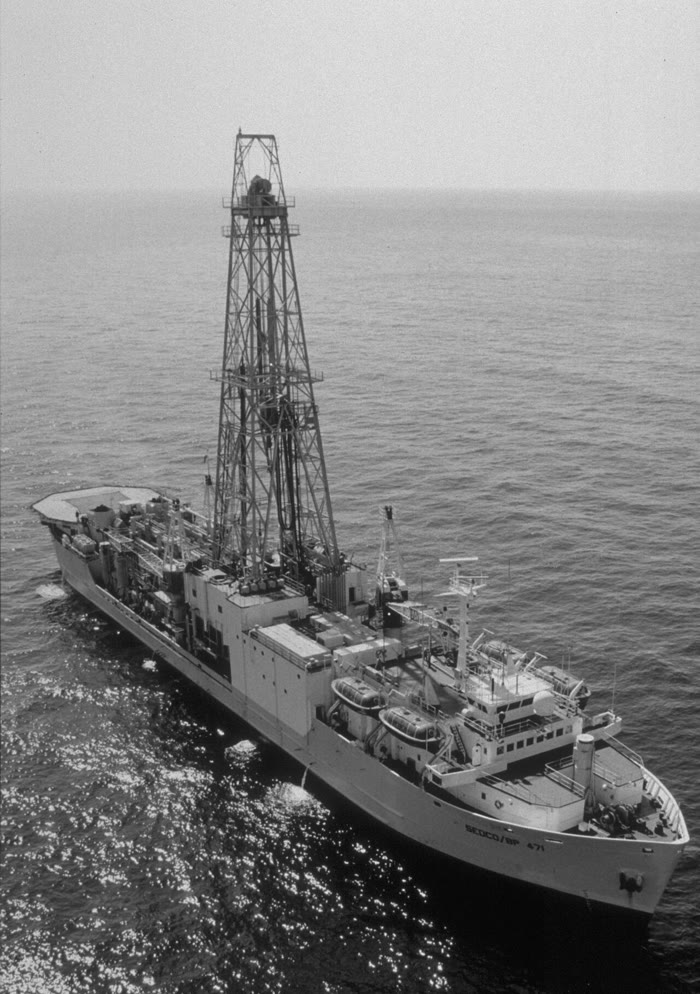
\includegraphics[width=0.36\linewidth]{images/book2/g11-odp-joides-resolution.jpg}

{\small سفينة الحفر \emph{«جويدس ريزولوشن»}، التي خلفت
\emph{«غلومار تشالنجر»}: البرج العالي هو برج الحفر فيها، وتحمل
السفينة أكثر من \qty{9000}{m} من أنابيب الحفر. الصورة: برنامج الحفر المحيطي، جامعة
تكساس للزراعة والميكانيكا (ملك عام).}
\end{omfigure}
% ledger: photo:g11-joides, usgs:glomar

منذ ذلك الحين، جُمعت آلاف المقاطع المغناطيسية ومئات آبار الحفر
في خريطة لعمر قاع المحيط كله.

\begin{omfigure}
\begin{tikzpicture}
\begin{axis}[ommap, width=\linewidth, xtick=\empty, ytick=\empty, grid=none,
    axis background/.style={}, clip=true, name=map]
  \addplot graphics[xmin=-180, xmax=180, ymin=-90, ymax=90] {figdata/out/grade-11-seafloor_age.png};
  \addplot[black!60, line width=0.15pt] table {figdata/out/shared-geo-land.dat};
\end{axis}
\begin{axis}[at={(map.south)}, anchor=north, yshift=-0.35cm, scale only axis, width=0.55\linewidth, height=0.32cm,
    xmin=0, xmax=200, ymin=0, ymax=1, axis y line=none, axis x line*=bottom,
    xtick={0,20,...,180}, tick label style={font=\scriptsize},
    xlabel={\foreignlanguage{arabic}{عمر قاع المحيط (بملايين السنين)؛ الرمادي: لا قاع محيطيًا}}, label style={font=\scriptsize},
    enlargelimits=false]
  \addplot graphics[xmin=0, xmax=200, ymin=0, ymax=1] {figdata/out/grade-11-seafloor_age-bar.png};
\end{axis}
\end{tikzpicture}

{\small عمر قاع المحيط. هو أحدث ما يكون (بالأحمر) على طول الظهرات، ثم يزداد
قِدمًا بالابتعاد عنها على الجانبين؛ ويقع أقدم القاع (بالأزرق والبنفسجي)
عند حواف المحيطات، قبالة القارات وعلى طول الخنادق.
البيانات: سيتون وآخرون (2020)، في خلايا من درجة واحدة؛ وحدود اليابسة:
Natural Earth.}
\end{omfigure}
% ledger: data:b2-seafloor-age, data:ne-land (map computed in figdata/grade-11/seafloor_age.py)

تؤكد الخريطة كل شيء دفعة واحدة. فعلى طول كل ظهرة يكون القاع حديثًا،
ويزداد عمره متماثلًا بالابتعاد عنها. ولا يوجد قاع محيطي أقدم من
نحو \num{190} مليون سنة: ويقع أقدمه في غرب المحيط الهادئ وقبالة
الساحل الشرقي لأمريكا الشمالية (وتُحسب على حدة بضعة أحواض صغيرة في شرق
البحر المتوسط). ومتوسط عمر قاع المحيط نحو
\num{64} مليون سنة، ونحو ثلاثة أرباعه أحدث من 100
مليون سنة --- في حين تحتفظ القارات بصخور أقدم بكثير. إن
قاع المحيط حديث لأنه يُصنع دائمًا عند الظهرات، ولأنه، كما
رأى هس، يُدمَّر في مكان آخر: أين؟ ذلك موضوع
\cref{ch:g11:subduction-zones}.
% ledger: data:b2-seafloor-age (oldest_open_myr 192.5, share_younger_100 0.76 in figdata/grade-11/seafloor_age.py), seton:mean-age, usgs:hess

\section{تمارين}

\begin{exercise}[$\star$]\label{exo:g11:drift-to-spreading:1}
عرّف \omterm{def:g11:drift-to-spreading:spreading}{توسع قاع المحيط}. ما الفرق بين \omterm{def:g11:drift-to-spreading:spreading-rate}{معدل التوسع الكلي}
ونصف \omterm{def:g11:drift-to-spreading:spreading-rate}{معدل التوسع} لظهرة ما؟
\end{exercise}

\begin{exercise}[$\star$]\label{exo:g11:drift-to-spreading:2}
لماذا لا تسجل اللابة اتجاه مجال الأرض إلا بعد أن تبرد
دون نحو \qty{580}{\celsius}؟ وماذا يحدث لذلك السجل إذا
سُخّن الصخر لاحقًا إلى \qty{700}{\celsius}؟
\end{exercise}

\begin{exercise}[$\star$]\label{exo:g11:drift-to-spreading:3}
يسمع مسبار صدى صدى نبضته بعد \qty{5.2}{s} من إرسالها.
إذا أُخذت سرعة الصوت في ماء البحر \qty{1500}{m/s}، فما عمق
قاع البحر؟
\end{exercise}

\begin{exercise}[$\star$]\label{exo:g11:drift-to-spreading:4}
على السلم الزمني للقطبية في هذا الفصل: كم دامت الفترة العادية
الحالية حتى الآن؟ وكم دام حدث هاراميو؟ وكم انقلابًا
حدث في آخر خمسة ملايين سنة؟
\end{exercise}

\begin{exercise}[$\star$]\label{exo:g11:drift-to-spreading:5}
يبلغ طول الظهرات وسط المحيطية نحو \qty{65000}{km}. ومحيط
الأرض نحو \qty{40000}{km}. كم مرة تلتف الظهرات
حول الأرض؟
\end{exercise}

\begin{exercise}[$\star\star$]\label{exo:g11:drift-to-spreading:6}
على مقطع مغناطيسي، يقع الحد بين فترتي برونهس وماتوياما
(\num{0.78} مليون سنة) على بعد \qty{20}{km} من محور الظهرة. احسب
نصف المعدل والمعدل الكلي بالسنتيمترات في السنة.
\end{exercise}

\begin{exercise}[$\star\star$]\label{exo:g11:drift-to-spreading:7}
على مقطع آخر، يقع حد غاوس--جلبرت (\num{3.58} مليون سنة) على بعد
\qty{45}{km} غرب المحور و\qty{44}{km} شرقه. احسب نصف المعدل على
كل جانب والمعدل الكلي. هل التوسع متماثل؟
\end{exercise}

\begin{exercise}[$\star\star$]\label{exo:g11:drift-to-spreading:8}
يقع الموقع 19 من حفريات عام 1968 على بعد \qty{990}{km} من محور
ظهرة وسط الأطلسي. باستعمال نصف معدل قدره \qty{1.9}{cm} في السنة، تنبأ
بعمر القاع هناك، وقارنه بعمر أقدم رواسبه البالغ \num{49}
مليون سنة.
\end{exercise}

\begin{exercise}[$\star\star$]\label{exo:g11:drift-to-spreading:9}
تتوسع ظهرة بنصف معدل قدره \qty{2}{cm} في السنة. باستعمال السلم الزمني في
هذا الفصل، أعط أبعاد الحدود التي أعمارها 0.78 و0.99 و1.07 و1.77 و1.95
مليون سنة عن المحور، وارسم الشرائط على جانب واحد،
والعادية منها بالأسود.
\end{exercise}

\begin{exercise}[$\star\star$]\label{exo:g11:drift-to-spreading:10}
متوسط عمر قاع المحيط نحو \num{64} مليون سنة؛ وعمر الأرض
نحو \num{4.6} مليار سنة. ما الكسر الذي يمثله ذلك من عمر الأرض؟
وأي حجج هس يدعم؟
\end{exercise}

\begin{exercise}[$\star\star$]\label{exo:g11:drift-to-spreading:11}
اشرح، مستعينًا برسم، لماذا يكون نمط الشرائط المغناطيسية على أحد جانبي
الظهرة صورة مرآة للنمط على الجانب الآخر. ما الذي قد يكسر
هذا التماثل؟
\end{exercise}

\begin{exercise}[$\star\star\star$]\label{exo:g11:drift-to-spreading:12}
لنفترض أن الظهرات، التي يبلغ طولها الكلي \qty{65000}{km}، تتوسع بمعدل كلي متوسط
قدره \qty{5}{cm} في السنة.
\begin{enumerate}
  \item ما مساحة قاع المحيط الجديد التي تصنعها كل سنة، بوحدة \unit{km^2}؟
  \item يغطي قاع المحيط نحو \qty{2.9e8}{km^2}. كم من الزمن تحتاج
        الظهرات لتصنع هذا القدر؟
  \item قارن بأقدم قاع محيطي، الذي يبلغ عمره نحو \num{190} مليون سنة.
        ماذا يجب أن يحدث لقاع المحيط بالسرعة نفسها التي يُصنع بها؟
\end{enumerate}
\end{exercise}

\begin{exercise}[$\star\star\star$]\label{exo:g11:drift-to-spreading:13}
دام حدث هاراميو من \num{0.99} إلى \num{1.07} مليون سنة مضت.
ما عرض شريطه على كل جانب من ظهرة نصف معدلها
\qty{1.25}{cm} في السنة، ومن أخرى نصف معدلها \qty{7.5}{cm} في السنة؟ يقع الصخر
الممغنط على عمق نحو \qty{3}{km} تحت سطح البحر. اشرح لماذا يظهر الحدث
بوضوح على المقطع السريع في هذا الفصل بينما لا يكاد يظهر على البطيء.
\end{exercise}

\begin{exercise}[$\star\star\star$]\label{exo:g11:drift-to-spreading:14}
في مواقع عام 1968، يبلغ سمك الرواسب \qty{176}{m} في الموقع 16، الذي يبلغ عمر قاعه
نحو \num{11} مليون سنة، ولا يتجاوز \qty{72}{m} في الموقع 20، الذي يبلغ عمره
نحو \num{67} مليون سنة. احسب المعدل المتوسط الذي
تراكمت به الرواسب في كل موقع، بالأمتار في كل مليون سنة. هل يمكن استعمال سمك
الرواسب لتأريخ القاع؟ وما الذي يُستعمل بدلًا منه؟
\end{exercise}

\begin{exercise}[$\star\star\star$]\label{exo:g11:drift-to-spreading:15}
على مقطع عبر ظهرة، يقع الحد الذي عمره \num{2.581} مليون سنة على بعد
\qty{58}{km} غرب المحور و\qty{70}{km} شرقه.
\begin{enumerate}
  \item احسب نصف المعدل على كل جانب والمعدل الكلي.
  \item لقد صُنع القاع شرق المحور أسرع من القاع غربه.
        بعد 10 ملايين سنة بهذين المعدلين، على أي بعد من المحور
        يقع القاع الذي له ذلك العمر على كل جانب؟
  \item اشرح لماذا تعطي المسافة بين الحدين المعدل
        الكلي حتى لو لم يكن التوسع متماثلًا.
\end{enumerate}
\end{exercise}

\section{مسألة: عمر جنوب الأطلسي}

\begin{problem}[{مسألة نهاية الأسبوع --- تأريخ محيط بثلاث طرق}]
\label{pb:g11:drift-to-spreading:1}
% ledger: dsdp3:table5, dsdp3:rate, data:b2-seafloor-age, earth:Rmean, ics:base.Cretaceous
% (values computed in figdata/grade-11/sediment_ages.py and seafloor_age.py)
في عام 1968 حفرت \emph{«غلومار تشالنجر»} سبع آبار عبر
ظهرة وسط الأطلسي قرب دائرة العرض \ang{30} جنوبًا. يعطي الجدول، لكل
موقع، بعده عن محور الظهرة، وعمر أقدم الرواسب على
البازلت (من أحافيرها)، وحيثما عُرف الشريط الذي تحته،
عمر ذلك الشريط المغناطيسي، بملايين السنين.

\begin{center}
\small
\begin{tabular}{|c|c|c|c|}
\hline
الموقع & البعد عن المحور (\unit{km}) & عمر أقدم الرواسب & عمر الشريط المغناطيسي \\ \hline
16 & 191 & 11 & 9 \\ \hline
15 & 380 & 24 & 21 \\ \hline
18 & 506 & 26 & --- \\ \hline
17 & 643 & 33 & --- \\ \hline
14 & 727 & 40 & 38.5 \\ \hline
19 & 990 & 49 & 53 \\ \hline
20 & 1270 & 67 & 71 \\ \hline
\end{tabular}

{\small البيانات: مشروع الحفر في أعماق البحار، الرحلة 3 (1970)؛ والأعمار المغناطيسية هي
منتصفات المجالات المعطاة هناك.}
\end{center}

\begin{center}
\begin{tikzpicture}
\begin{axis}[omrecord, width=0.82\linewidth, height=5.0cm, xmin=-50, xmax=16, ymin=0, ymax=140,
  xlabel={\foreignlanguage{arabic}{خط الطول على امتداد \babelsublr{\ang{30}} جنوبًا، بالدرجات؛ السالب: غربًا}}, ylabel={\foreignlanguage{arabic}{العمر بملايين السنين}},
  tick label style={font=\small}, label style={font=\small}, clip=false]
\addplot[omDef, line width=0.8pt] table[x=lon, y=age] {figdata/out/grade-11-seafloor_age-profile.dat};
\draw[omRidge, densely dashed] (axis cs:-13.8,0) -- (axis cs:-13.8,140);
\node[font=\scriptsize, text=omRidge, anchor=south] at (axis cs:-13.8,140) {محور الظهرة};
\fill (axis cs:-47.4,125.1) circle (1.5pt);
\node[font=\scriptsize, anchor=south west, inner sep=2pt] at (axis cs:-47.6,126) {أمريكا الجنوبية};
\node[font=\scriptsize, anchor=north west, align=left] at (axis cs:14.2,135) {إفريقيا};
\fill (axis cs:13.8,129.8) circle (1.5pt);
\end{axis}
\end{tikzpicture}

{\small عمر قاع المحيط على امتداد دائرة العرض \ang{30} جنوبًا، من
أمريكا الجنوبية إلى إفريقيا؛ ويتوقف الخط حيث ينتهي قاع المحيط قبالة
كل قارة. البيانات: سيتون وآخرون (2020).}
\end{center}

\medskip
\noindent\textbf{الجزء الأول --- مواقع الحفر.}
\begin{enumerate}
  \item أي المواقع أقرب إلى الظهرة، وأيها أبعد؟ وكيف
        يقارن عمراهما؟
  \item لماذا يكون عمر أقدم الرواسب الواقعة على البازلت قريبًا من
        عمر البازلت نفسه؟ هل هو أقدم قليلًا أم أحدث
        قليلًا؟
  \item احسب لكل موقع نسبة بعده إلى عمر أقدم
        رواسبه، بالكيلومترات في كل مليون سنة.
  \item ما متوسط هذه النسب السبع؟ حوّله إلى سنتيمترات في
        السنة.
  \item يقع الموقعان 17 و18 شرق الظهرة، والمواقع الأخرى غربها. هل
        تتبع المواقع الشرقية الاتجاه نفسه الذي تتبعه الغربية؟ وماذا يدل
        ذلك على التوسع؟
\end{enumerate}

\medskip
\noindent\textbf{الجزء الثاني --- المعدل من الرواسب.}
\begin{enumerate}[resume]
  \item لو توسع القاع بنصف معدل ثابت $u$، فكيف يتوقف عمر
        القاع $t$ على بعده $d$ عن المحور؟
  \item ميل المستقيم المار بالأصل الذي يلائم النقاط على أفضل وجه هو
        $u = \sum d\,t / \sum t^2$. وللمواقع السبعة،
        $\sum d\,t = \num{208276}$ و$\sum t^2 = \num{10952}$ (بالكيلومترات
        وملايين السنين). احسب $u$ بالكيلومترات في كل
        مليون سنة وبالسنتيمترات في السنة.
  \item ما \omterm{def:g11:drift-to-spreading:spreading-rate}{معدل التوسع الكلي} لجنوب الأطلسي عند دائرة العرض
        هذه؟
  \item كتب علماء البعثة أن المعدل «أقل قليلًا
        من \qty{2}{cm} في السنة». هل توافقهم؟
  \item بهذا المعدل، تنبأ بعمر القاع في الموقع 20، وقارنه
        بعمر أقدم رواسبه.
\end{enumerate}

\medskip
\noindent\textbf{الجزء الثالث --- المعدل من الشرائط المغناطيسية.}
\begin{enumerate}[resume]
  \item من الموقع 16 وحده (\qty{191}{km}، شريط عمره 9 ملايين سنة)،
        احسب نصف معدل.
  \item من الموقع 20 وحده (\qty{1270}{km}، شريط عمره 71 مليون سنة)،
        احسب نصف معدل.
  \item للمواقع الخمسة التي لها عمر مغناطيسي، $\sum d\,t = \num{180329}$
        و$\sum t^2 = \num{9854}$. احسب أفضل نصف معدل.
  \item بكم في المئة يختلف المعدل المستخرج من الأحافير عن المستخرج من
        الشرائط؟ هل تتفق الطريقتان؟
  \item لماذا من المهم أن العمرين وُجدا بطريقتين
        مختلفتين تمامًا؟
\end{enumerate}

\medskip
\noindent\textbf{الجزء الرابع --- إلى حافة المحيط.}
\begin{enumerate}[resume]
  \item على امتداد دائرة العرض \ang{30} جنوبًا، يقع محور الظهرة عند خط الطول
        \ang{13.8} غربًا وينتهي قاع المحيط قبالة إفريقيا عند
        \ang{13.8} شرقًا. كم درجة من خطوط الطول تفصل بينهما؟
  \item على كرة نصف قطرها \qty{6371}{km}، يبلغ طول درجة واحدة من خط الطول
        $\qty{111.2}{km} \times \cos(\text{دائرة العرض})$. احسب
        طول درجة واحدة عند \ang{30} جنوبًا، والمسافة من
        المحور إلى حافة قاع المحيط بجوار إفريقيا.
  \item لو توسع القاع دائمًا بمعدل الجزء الثاني، فمنذ متى
        يكون القاع عند الحافة قد تكوّن؟
  \item تعطي خريطة الأعمار، التي تؤرخ القاع القديم بشرائطه المغناطيسية،
        \num{130} مليون سنة عند الحافة. ما نصف المعدل المتوسط الذي
        يقتضيه ذلك؟ هل كان الانفتاح المبكر للمحيط أسرع قليلًا أم
        أبطأ قليلًا من انفتاح آخر 66 مليون سنة؟
  \item استنتج: ما عمر أقدم قاع محيطي بجوار إفريقيا عند
        \ang{30} جنوبًا؟ بدأ العصر الطباشيري قبل نحو \num{143} مليون
        سنة: ففي أي عصر بدأ جنوب الأطلسي ينفتح
        هناك؟
\end{enumerate}
\end{problem}
